\begin{frame}[fragile]
\frametitle{Aufbau und Modell}

\begin{center}
		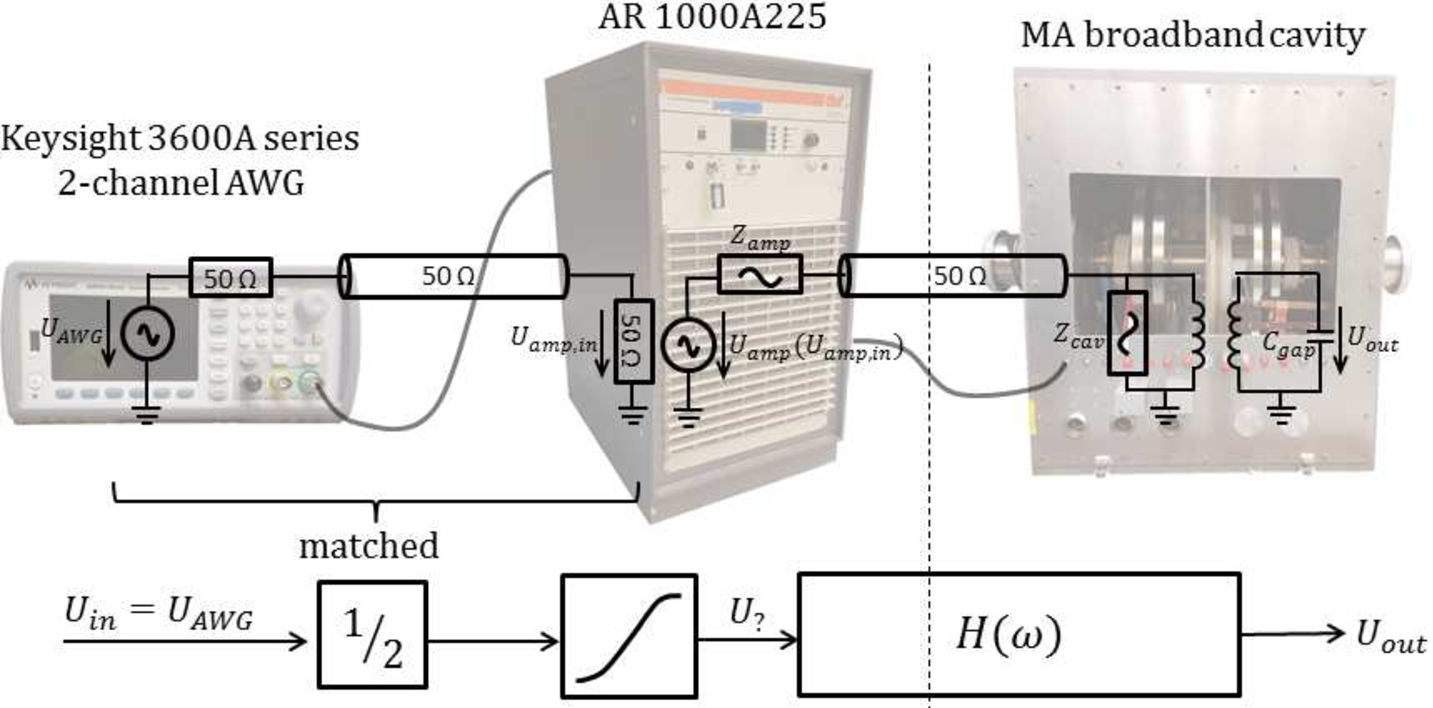
\includegraphics[scale=0.45]{slides/ResultCode/WEPVA047f2_2-eps-converted-to.pdf} 
	\end{center}
\end{frame}

\begin{frame}[fragile]
\frametitle{Aufbau und Modell}

	
	{
	\begin{itemize}
	\item Hammerstein Modell \uncover<2-> {: 
		\begin{itemize}
			\item System ist linear bis $\hat{U}_{BB} \approx 550V$
			\item Ergänzung um eine nichtlineare Vorverzerrung
			\item Potenzreihenansatz $U_?(t)=\sum_{n=1}^N a_n \left[ U_{in}(t) \right]^n$
		\end{itemize}
		}
	\item Zielsetzung \uncover<3-> {:
		\begin{itemize}
			\item Parameter $a_n$ der Kennlinie zubestimmen
		\end{itemize}
		}
	 \end{itemize}
	}
	\centering
	\begin{picture}(100,70)
		\put(15,5){
			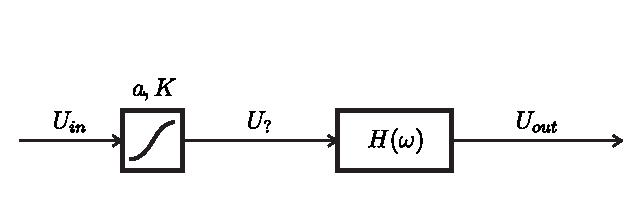
\includegraphics[scale=1.0]{slides/ResultCode/Slide1.eps} 
		}
	\end{picture}
%\begin{picture}(100,70)
%		\put(15,0){
%			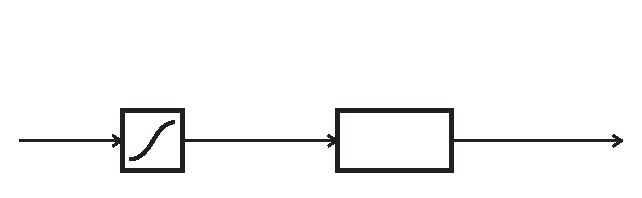
\includegraphics[scale=1.0]{slides/ResultCode/Slide2.eps} 
%		}  
%	\end{picture}
\end{frame}
